
\subsubsection[Centroid-based (K-means)]{Centroid-based \textit{(K-means)}}
\begin{frame}

	\frametitle{{\color{GradientDescentDiagramBlue}Centroid-based Clustering}, in sintesi}

	%\begin{block}{}
		Il \textbf{centroid-based clustering} organizza i dati in cluster non gerarchici, in contrasto con il clustering gerarchico definito in seguito. \textbf{K-means} è l'algoritmo di clustering basato su centroidi più utilizzato.
		\newlinedouble
		Gli algoritmi basati su centroidi sono efficienti ma \textbf{sensibili} alle \textbf{condizioni iniziali} e ai \textbf{valori anomali}.

		\begin{figure}[!htbp]
			\centering
			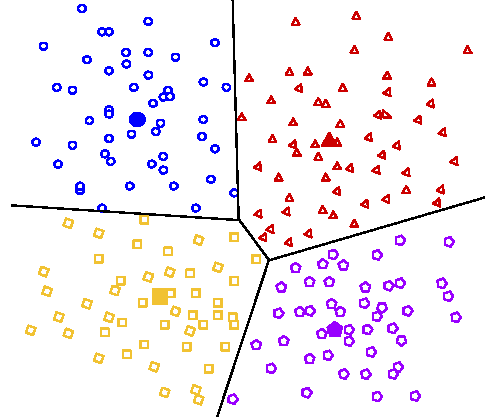
\includegraphics[width=5.0cm]{images/unsupervised/types/Clustering_CentroidBased.pdf}
					%\caption{Stripe Radar for Fraud Detection}
		\end{figure}
	%\end{block}

\end{frame}



\begin{frame}

	\frametitle{{\color{GradientDescentDiagramBlue}Centroid-based Clustering}: il K-means}

	\begin{scriptsize}
	\begin{block}{Come calcolare la media $\mu$ per un insieme di punti $\in \mathbb{R}^1$}
		\begin{figure}[!htbp]
			\centering
			\includegraphics<1>[width=0.7\linewidth]{images/unsupervised/kmeans/mean_r1.png}
			\includegraphics<2>[width=0.7\linewidth]{images/unsupervised/kmeans/mean_r1_mean.png}
					%\caption{Stripe Radar for Fraud Detection}
		\end{figure}
		
		\begin{itemize}
	        \item<1-> $\mu = \frac{2+3+7+8}{4} = 5$	       
	        \item<2-> $\mu = \frac{x_1 + x_2 + ... + x_N}{N} = \frac{1}{N}\sum_{i=1}^{N} x_i$
	    \end{itemize}

	\end{block}
	\end{scriptsize}
	
\end{frame}

\begin{frame}

	\frametitle{{\color{GradientDescentDiagramBlue}Centroid-based Clustering}: il K-means}

	\begin{scriptsize}
	\begin{block}{Come calcolare la media $\mu$ per un insieme di punti $\in \mathbb{R}^2$}
		\begin{figure}[!htbp]
			\centering
			\includegraphics<1>[width=0.56\linewidth]{images/unsupervised/kmeans/mean_r2.png}
			\includegraphics<2>[width=0.56\linewidth]{images/unsupervised/kmeans/mean_r2_mean.png}
					%\caption{Stripe Radar for Fraud Detection}
		\end{figure}
		
		\begin{align}
			\bar \mu = (\mu_1, \mu_2) &= \left(\frac{2+3+7+8}{4}, \frac{1+0+1+2}{4}\right) = (5,1)\nonumber \\
			\bar \mu = (\mu_1, \mu_2) &= \frac{1}{4} \left[(2,1) + (3,0) + (7,1) + (8,2)\right] \nonumber \\
			& = \frac{1}{4} (20, 4) \nonumber \\
			& = (5,1) \nonumber
		\end{align}
	\end{block}
	\end{scriptsize}
	
\end{frame}


\begin{frame}

	\frametitle{{\color{GradientDescentDiagramBlue}Centroid-based Clustering}: il K-means}
	
	\begin{scriptsize}
	\begin{block}{Come calcolare la media $\mu$ per un insieme di punti $\in \mathbb{R}^2$}
		\begin{figure}[!htbp]
			\centering
			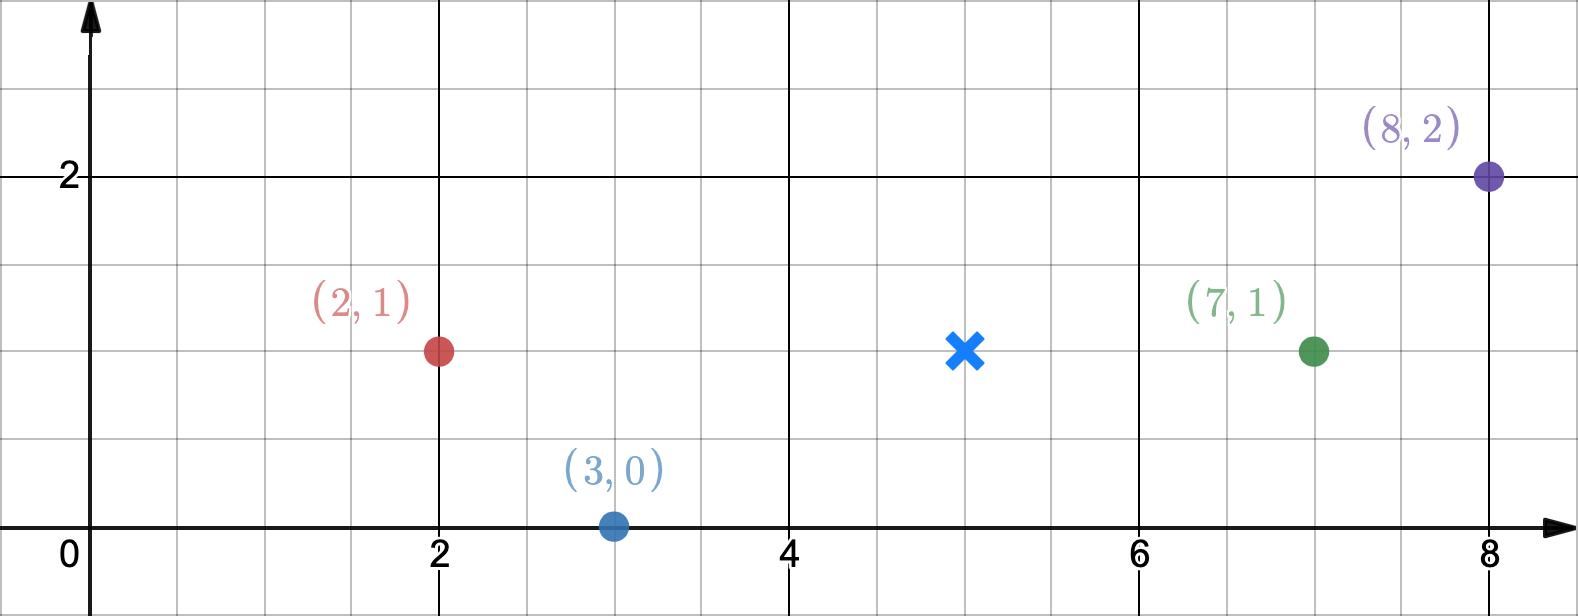
\includegraphics[width=0.5\linewidth]{images/unsupervised/kmeans/mean_r2_mean.png}
					%\caption{Stripe Radar for Fraud Detection}
		\end{figure}
		
		$$\bar \mu = (\mu_1, \mu_2) = \frac{1}{N} (\bar x_1 + \bar x_2 + ... + \bar x_N) = \frac{1}{N}\sum_{i=1}^{N} \bar x_i$$

	\end{block}
	
	\begin{block}{Come calcolare la media $\mu$ per un insieme di punti $\in \mathbb{R}^D$}
		$$\bar \mu = (\mu_1, \mu_2, ..., \mu_D) = \frac{1}{N} (\bar x_1 + \bar x_2 + ... + \bar x_N) = \frac{1}{N}\sum_{i=1}^{N} \bar x_i$$
	\end{block}
	\end{scriptsize}

\end{frame}




\begin{frame}

	\frametitle{{\color{GradientDescentDiagramBlue}Centroid-based Clustering}: il K-means}

	%\begin{block}{}
		Il clustering \textbf{K-means} è caratterizzato dai seguenti aspetti chiave:
		\begin{itemize}
			\item con il clustering K-means, il \textbf{numero K} di cluster deve essere specificato prima di iniziare il processo di clustering
			\item il clustering K-means \textbf{non è gerarchico}: il dataset è semplicemente partizionato in \textbf{K gruppi disgiunti}
			\ifthenelse{\boolean{highschool}}{}{
				\item K-means scala come $O(nk)$, dove $k$ è il numero di clusters e $n$ la dimensione del dataset
			}
		\end{itemize}
		
		\pause
		\vspace{2em}
		Definiamo la variabile binaria $r_{ik}$ che vale:
		\begin{itemize}
			\item 1: se l'$i$-esima osservazione $\in$ al cluster $k$
			\item 0: altrimenti
		\end{itemize}
		Ogni osservazione può essere assegnata ad un solo cluster, di conseguenza per ogni singola osservazione $i$ esisterà una e una sola $\hat{k}$ per il quale vale che  $r_{i\hat{k}}=1$.

	%\end{block}

\end{frame}



\begin{frame}

	\frametitle{{\color{GradientDescentDiagramBlue}Centroid-based Clustering}: il K-means}

	\begin{block}{K-means: algoritmo}
		\begin{enumerate}
			\item inizializza in modo casuale i valori delle variabili binarie $r_{ik}$ in modo che ogni punto sia assegnato casualmente ad un solo cluster 
			\item calcola la media di ogni cluster (cioè il centro del cluster):\\
				$\mu_k = \frac{\sum_{i=1}^{N}r_{ik}x_i}{\sum_{i=1}^{N}r_{ik}} =$ (la media delle osservazioni appartenti al cluster $k$)
			\item aggiorna i valori delle variabili binarie $r_{ik}$, in modo che ogni punto sia assegnato al centro del cluster più vicino
			\item se nessuna variabile viene aggiornata nel passaggio precedente, fermarsi, altrimenti tornare al passaggio 2
		\end{enumerate}
		\vspace{2mm}
		Una possibile inizializzazione alternativa prevede di fissare direttamente i centri dei clusters randomicamente (ad esempio scegliendo $k$ distinti punti random dal dataset) e poi procedere dal punto 3
	\end{block}

\end{frame}


\begin{frame}

	\frametitle{{\color{GradientDescentDiagramBlue}Centroid-based Clustering}: il K-means}

	\begin{block}{K-means: algoritmo}
		\begin{figure}[!htbp]
			\centering
			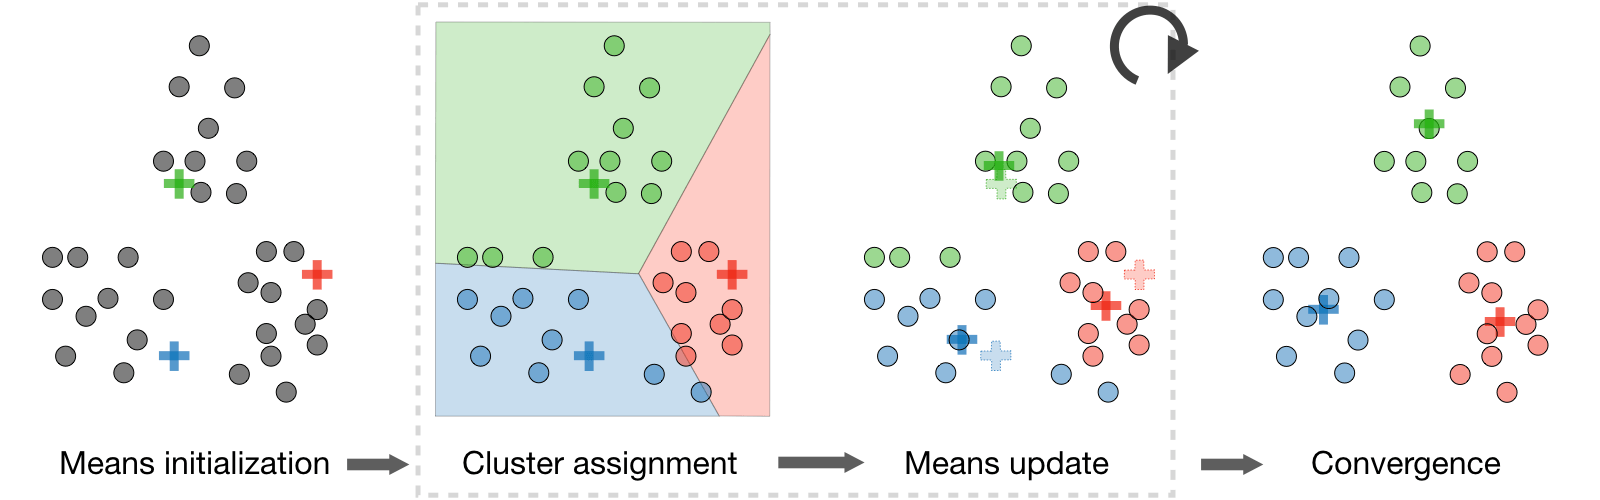
\includegraphics[width=1.0\linewidth]{images/unsupervised/kmeans/kmeans_algorithm.png}
					%\caption{Stripe Radar for Fraud Detection}
		\end{figure}
	\end{block}

\end{frame}


%\begin{frame}
%
%	\frametitle{{\color{GradientDescentDiagramBlue}Centroid-based Clustering}: il K-means}
%
%	\begin{block}{K-means: algoritmo\\Inizializzazione alternativa}
%		\begin{figure}[!htbp]
%			\centering
%			\includegraphics[width=5.75cm]{images/unsupervised/kmeans/kmeans_step_1.png}
%					%\caption{Stripe Radar for Fraud Detection}
%		\end{figure}
%	\end{block}
%
%\end{frame}
%
%
%\begin{frame}
%
%	\frametitle{{\color{GradientDescentDiagramBlue}Centroid-based Clustering}: il K-means}
%
%	\begin{block}{K-means: algoritmo\\Aggiorno gli $r_{ik}\text{ }$(punto 3)}
%		\begin{figure}[!htbp]
%			\centering
%			\includegraphics[width=5.75cm]{images/unsupervised/kmeans/kmeans_step_2.png}
%					%\caption{Stripe Radar for Fraud Detection}
%		\end{figure}
%	\end{block}
%
%\end{frame}
%
%
%\begin{frame}
%
%	\frametitle{{\color{GradientDescentDiagramBlue}Centroid-based Clustering}: il K-means}
%
%	\begin{block}{K-means: algoritmo\\La condizione di stop non è ancora rispettata quindi aggiorno i $\mu_k$ (punto 2)}
%		\begin{figure}[!htbp]
%			\centering
%			\includegraphics[width=5.75cm]{images/unsupervised/kmeans/kmeans_step_3.png}
%					%\caption{Stripe Radar for Fraud Detection}
%		\end{figure}
%	\end{block}
%
%\end{frame}
%
%
%\begin{frame}
%
%	\frametitle{{\color{GradientDescentDiagramBlue}Centroid-based Clustering}: il K-means}
%
%	\begin{block}{K-means: algoritmo\\Aggiorno gli $r_{ik}\text{ }$(punto 3)}
%		\begin{figure}[!htbp]
%			\centering
%			\includegraphics[width=5.75cm]{images/unsupervised/kmeans/kmeans_step_4.png}
%					%\caption{Stripe Radar for Fraud Detection}
%		\end{figure}
%	\end{block}
%
%\end{frame}


\begin{frame}

	\frametitle{{\color{GradientDescentDiagramBlue}Centroid-based Clustering}: il K-means}

%	\begin{block}{K-means: algoritmo}
		\centering
		\animategraphics[controls={play, step, stop}, height=7cm]{20.0}{images/unsupervised/kmeans/k_means_1/k_means_1-}{0}{242}
%	\end{block}

\end{frame}


\begin{frame}

	\frametitle{{\color{GradientDescentDiagramBlue}Centroid-based Clustering}: il K-means}

%	\begin{block}{K-means: algoritmo}
		\centering
		\animategraphics[controls={play, step, stop}, height=7cm]{3.0}{images/unsupervised/kmeans/k_means_2/k_means_2-}{0}{14}
%	\end{block}

\end{frame}


\begin{frame}

	\frametitle{{\color{GradientDescentDiagramBlue}Centroid-based Clustering}: il K-means}

%	\begin{block}{K-means: algoritmo}
		\centering
		\animategraphics[controls={play, step, stop}, height=7cm]{3.0}{images/unsupervised/kmeans/k_means_3/k_means_3-}{0}{12}
%	\end{block}

\end{frame}


\begin{frame}

	\frametitle{{\color{GradientDescentDiagramBlue}Centroid-based Clustering}: il K-means}

	\begin{block}{}
		Per altri esempi interattivi:\\
		\begin{itemize}
			\item \underline{\href{https://stanford.edu/class/engr108/visualizations/kmeans/kmeans.html}{Esempio 1}}
			\item \underline{\href{http://alekseynp.com/viz/k-means.html}{Esempio 2}}
		\end{itemize}
	\end{block}

\end{frame}


\ifthenelse{\boolean{highschool}}{}{
	\begin{frame}
	
		\frametitle{{\color{GradientDescentDiagramBlue}Centroid-based Clustering}: il K-means}
	
		\begin{block}{K-means: dimostrazione matematica parte 1}
			Ricordiamo l'espressione di:
			\begin{empheq}[box=\fcolorbox{blue!40!black!60}{yellow!10}]{align*}
				\mathbf{J} = \frac{1}{N} \sum_{i=1}^{N}\sum_{k=1}^{K}r_{ik} \Vert x_i-\mu_k\Vert^2
			\end{empheq}
	
			Dati $N$ esempi assegnati a $K$ cluster, minimizziamo la somma delle distanze degli esempi rispetto ai loro centroidi. Dove:
			\begin{itemize}
				\item $r_{ik}=1$ quando l'$i$-esimo esempio è assegnato al $k$-esimo cluster, $=0$ altrimenti
				\item $\mu_k$ è il centroide del $k$-esimo cluster
			\end{itemize}
		\end{block}
	
	\end{frame}
	
	
	\begin{frame}
	
		\frametitle{{\color{GradientDescentDiagramBlue}Centroid-based Clustering}: il K-means}
	
		\begin{block}{K-means: dimostrazione matematica parte 2}
	
			Vogliamo quindi minimizzare la seguente espressione:
			$$\underset{r,\mu}{min}\sum_{i=1}^{N}\sum_{k=1}^{K}r_{ik} \Vert x_i-\mu_k\Vert^2$$
			dove:
			$$r_{ik} \in \{0,1\}\quad\forall i,k$$
			e
			$$\sum^{K}_{k=1}r_{ik}=1\quad\forall i$$
	
			Per minimizzare l'espressione rispetto al cluster con centroide $\mu_k$, deriviamo rispetto a $\mu_k$ e la uguagliamo a 0.
		\end{block}
	
	\end{frame}
	
	
	\begin{frame}
	
		\frametitle{{\color{GradientDescentDiagramBlue}Centroid-based Clustering}: il K-means}
	
		\begin{block}{K-means: dimostrazione matematica parte 3}
			
			\begin{center}
				$f(\mu) = \sum^{N}_{i=1} \sum_{k=1}^{K} r_{ik} ||x_i - \mu_k||^2$ \newlinedouble %\hline
				$\frac{\partial f}{\partial \mu_k} = 2 \sum_{i=1}^{N} r_{ik}(x_i - \mu_k) = 0$  \\~\\ $\pmb{\Downarrow}$ \\~\\
				 %\hline
				$\quad \sum_{i=1}^{N} r_{ik}\mu_{k} = \sum_{i=1}^{N} r_{ik}x_{i}$ \newlinedouble %\hline
				$\mu_k \sum_{i=1}^{N} r_{ik} = \sum_{i=1}^{N} r_{ik} x_i$ \newlinedouble %\hline
				$\mu_k = \frac{\sum_{i=1}^{N} r_{ik} x_i}{\sum_{i=1}^{N} r_{ik}}$	
			\end{center}
	
		\end{block}
	
	\end{frame}
	
	
	\begin{frame}
	
		\frametitle{{\color{GradientDescentDiagramBlue}Centroid-based Clustering}: il K-means}
	
		\begin{block}{K-means: dimostrazione matematica parte 4}
	
	%		\begin{scriptsize}
				\begin{gather*}
					 \mu_k = \frac{\sum_{i=1}^{N} r_{ik} x_i}{\sum_{i=1}^{N} r_{ik}}
				\end{gather*}
	%		\end{scriptsize}
	
			\begin{itemize}
				\item il \textbf{numeratore} è la somma di tutti i  punti (vettori) appartenti al cluster
				\item il \textbf{denominatore} è il numero di esempi nel cluster
				\item pertanto, il centroide del cluster $\mu_k$ è la media delle posizioni dei punti appartenenti al cluster
				\item quindi in estrema sintesi: per minimizzare $J$ è sufficiente aggiornare il $\mu_k$ del cluster sommando i vari vettori (punti) del cluster e dividere per il numero di elementi del cluster (media di tutti i punti nel cluster)
			\end{itemize}
	
		\end{block}
	
	\end{frame}
}


\begin{frame}

	\frametitle{{\color{GradientDescentDiagramBlue}Centroid-based Clustering}: il K-means}

	\begin{block}{K-means: svantaggi}
		\begin{itemize}
			\item uno svantaggio del clustering k-means è che non è garantito che converga sempre allo stesso clustering
				\begin{itemize}
					\item[--] l'esecuzione della procedura più volte può produrre cluster diversi: a seconda dell'inizializzazione randomica l'algoritmo può convergere a minimi (locali) diversi
				\end{itemize}
			\item un altro svantaggio è che l'uso della distanza euclidea determina cluster sferici
		\end{itemize}
	\end{block}

\end{frame}


\begin{frame}

	\frametitle{{\color{GradientDescentDiagramBlue}Centroid-based Clustering}: il K-means}

	\begin{block}{K-means: minimi locali diversi parte 1}
		\begin{itemize}
			\item Considera il seguente dataset composto da punti 2D appartenenti a 2 classi distinte
			\item ogni classe è caratterizzata da una distribuzione gaussiana (parzialmente sovrapposta)
		\end{itemize}

		\begin{figure}[!htbp]
			\centering
			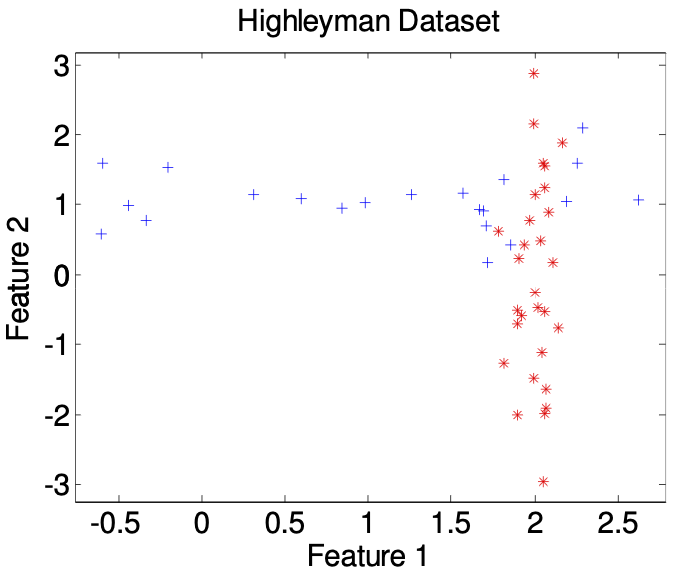
\includegraphics[width=4.50cm]{images/unsupervised/kmeans/highley_gt.png}
					%\caption{Stripe Radar for Fraud Detection}
		\end{figure}
	\end{block}

\end{frame}


\begin{frame}

	\frametitle{{\color{GradientDescentDiagramBlue}Centroid-based Clustering}: il K-means}

	\begin{block}{K-means: minimi locali diversi parte 2}
		Risultato usando K-means con $K=2$
		\begin{columns}
			\column{0.5\linewidth}
			\begin{figure}[!htbp]
				\centering
				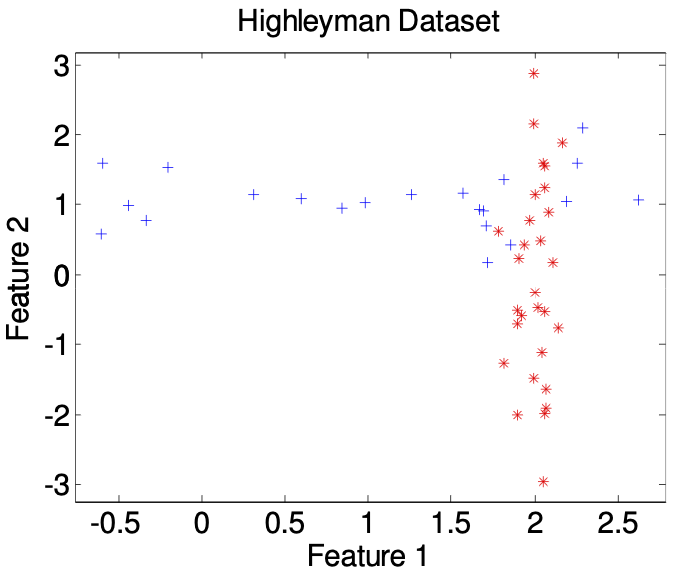
\includegraphics[angle=0,width=1\linewidth]{images/unsupervised/kmeans/highley_gt.png}
%				\caption{Single-Link Good K}
				%\label{Enel_HistFit_Normal}
			\end{figure}

			\column{0.5\linewidth}
			\begin{figure}[!htbp]
				\centering
				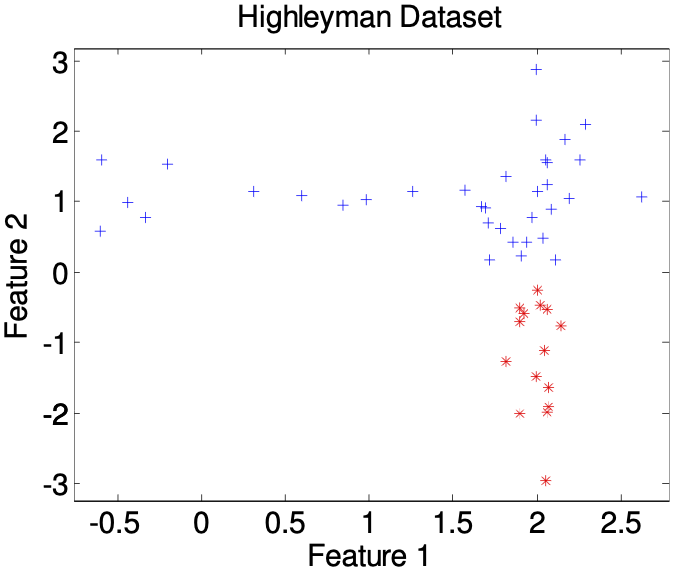
\includegraphics[angle=0,width=1\linewidth]{images/unsupervised/kmeans/highley_2k.png}
%				\caption{Single-Link Dendogram Good K}
				%\label{Enel_QQ_Plot_Normal}
			\end{figure}

		\end{columns}
	\end{block}

\end{frame}



\begin{frame}

	\frametitle{{\color{GradientDescentDiagramBlue}Centroid-based Clustering}: il K-means}

	\begin{block}{K-means: minimi locali diversi parte 3}
		Risultato 1 usando K-means con $K=3$
		\begin{columns}
			\column{0.5\linewidth}
			\begin{figure}[!htbp]
				\centering
				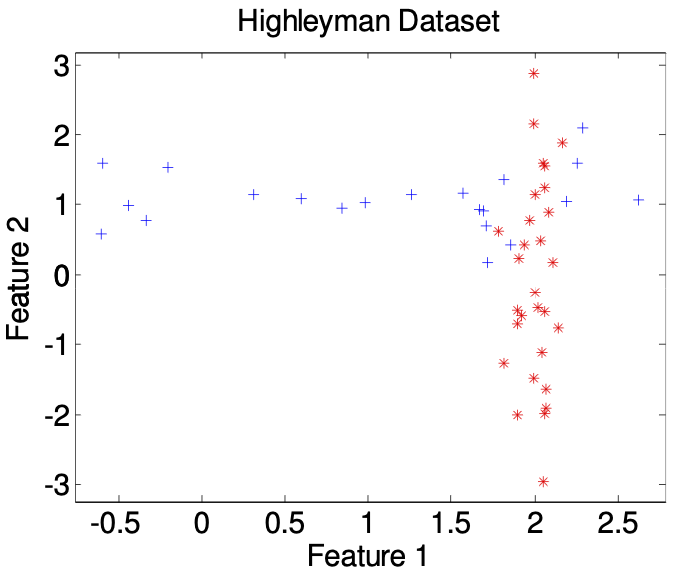
\includegraphics[angle=0,width=1\linewidth]{images/unsupervised/kmeans/highley_gt.png}
%				\caption{Single-Link Good K}
				%\label{Enel_HistFit_Normal}
			\end{figure}

			\column{0.5\linewidth}
			\begin{figure}[!htbp]
				\centering
				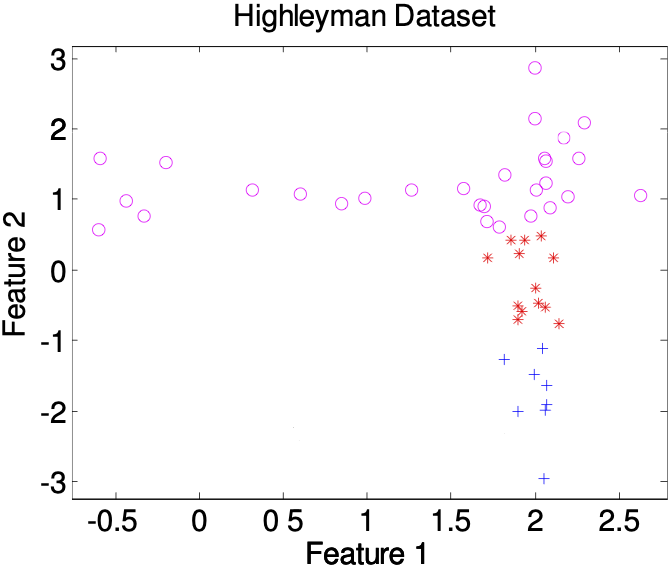
\includegraphics[angle=0,width=1\linewidth]{images/unsupervised/kmeans/highley_3k_1.png}
%				\caption{Single-Link Dendogram Good K}
				%\label{Enel_QQ_Plot_Normal}
			\end{figure}

		\end{columns}
	\end{block}

\end{frame}


\begin{frame}

	\frametitle{{\color{GradientDescentDiagramBlue}Centroid-based Clustering}: il K-means}

	\begin{block}{K-means: minimi locali diversi parte 4}
		Risultato 2 usando K-means con $K=3$
		\begin{columns}
			\column{0.5\linewidth}
			\begin{figure}[!htbp]
				\centering
				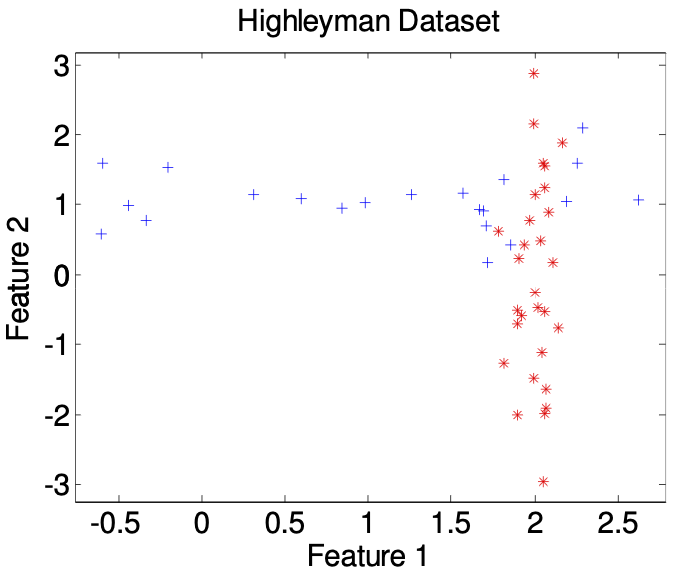
\includegraphics[angle=0,width=1\linewidth]{images/unsupervised/kmeans/highley_gt.png}
%				\caption{Single-Link Good K}
				%\label{Enel_HistFit_Normal}
			\end{figure}

			\column{0.5\linewidth}
			\begin{figure}[!htbp]
				\centering
				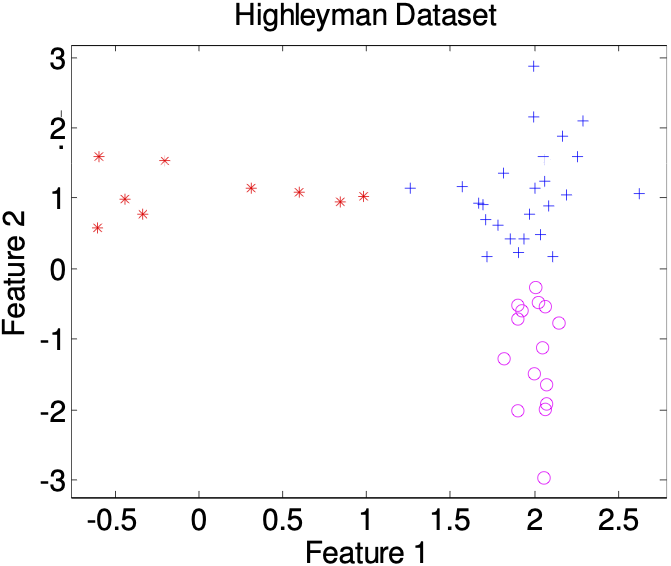
\includegraphics[angle=0,width=1\linewidth]{images/unsupervised/kmeans/highley_3k_2.png}
%				\caption{Single-Link Dendogram Good K}
				%\label{Enel_QQ_Plot_Normal}
			\end{figure}

		\end{columns}
	\end{block}

\end{frame}


\begin{frame}

	\frametitle{{\color{GradientDescentDiagramBlue}Centroid-based Clustering}: considerazioni}

	%\begin{block}{K-means: considerazioni}

		\begin{itemize}
			\item La procedura iterativa K-means cerca di spostare i centri del cluster in modo da farli corrispondere a posizioni nello spazio delle features in cui si concentrano molti punti
				\begin{itemize}
					\item[--] idealmente, i centri dei cluster dovrebbero essere posizionati in corrispondenza dei \textbf{picchi della densità} di distribuzione dei dati nello spazio delle features
				\end{itemize}
			\item Un risultato dell'utilizzo della distanza euclidea per valutare la vicinanza di un punto dati al centro del suo cluster è che la forma di ciascun cluster rappresenta una cella Voronoi
				\begin{itemize}
					\item[--] l'insieme di tutti i cluster determina una \textbf{tassellazione Voronoi} del spazio delle caratteristiche
				\end{itemize}
		\end{itemize}

		\begin{figure}[!htbp]
				\centering
				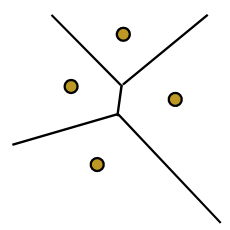
\includegraphics[angle=0,width=0.18\linewidth]{images/unsupervised/kmeans/kmeans_voronoi.png}
%				\caption{Single-Link Dendogram Good K}
				%\label{Enel_QQ_Plot_Normal}
			\end{figure}
	%\end{block}

\end{frame}


\begin{frame}

	\frametitle{{\color{GradientDescentDiagramBlue}Centroid-based Clustering}: segmentazione con il K-means}

%	\begin{block}{K-means: considerazioni}
		\begin{figure}[!htbp]
			\centering
			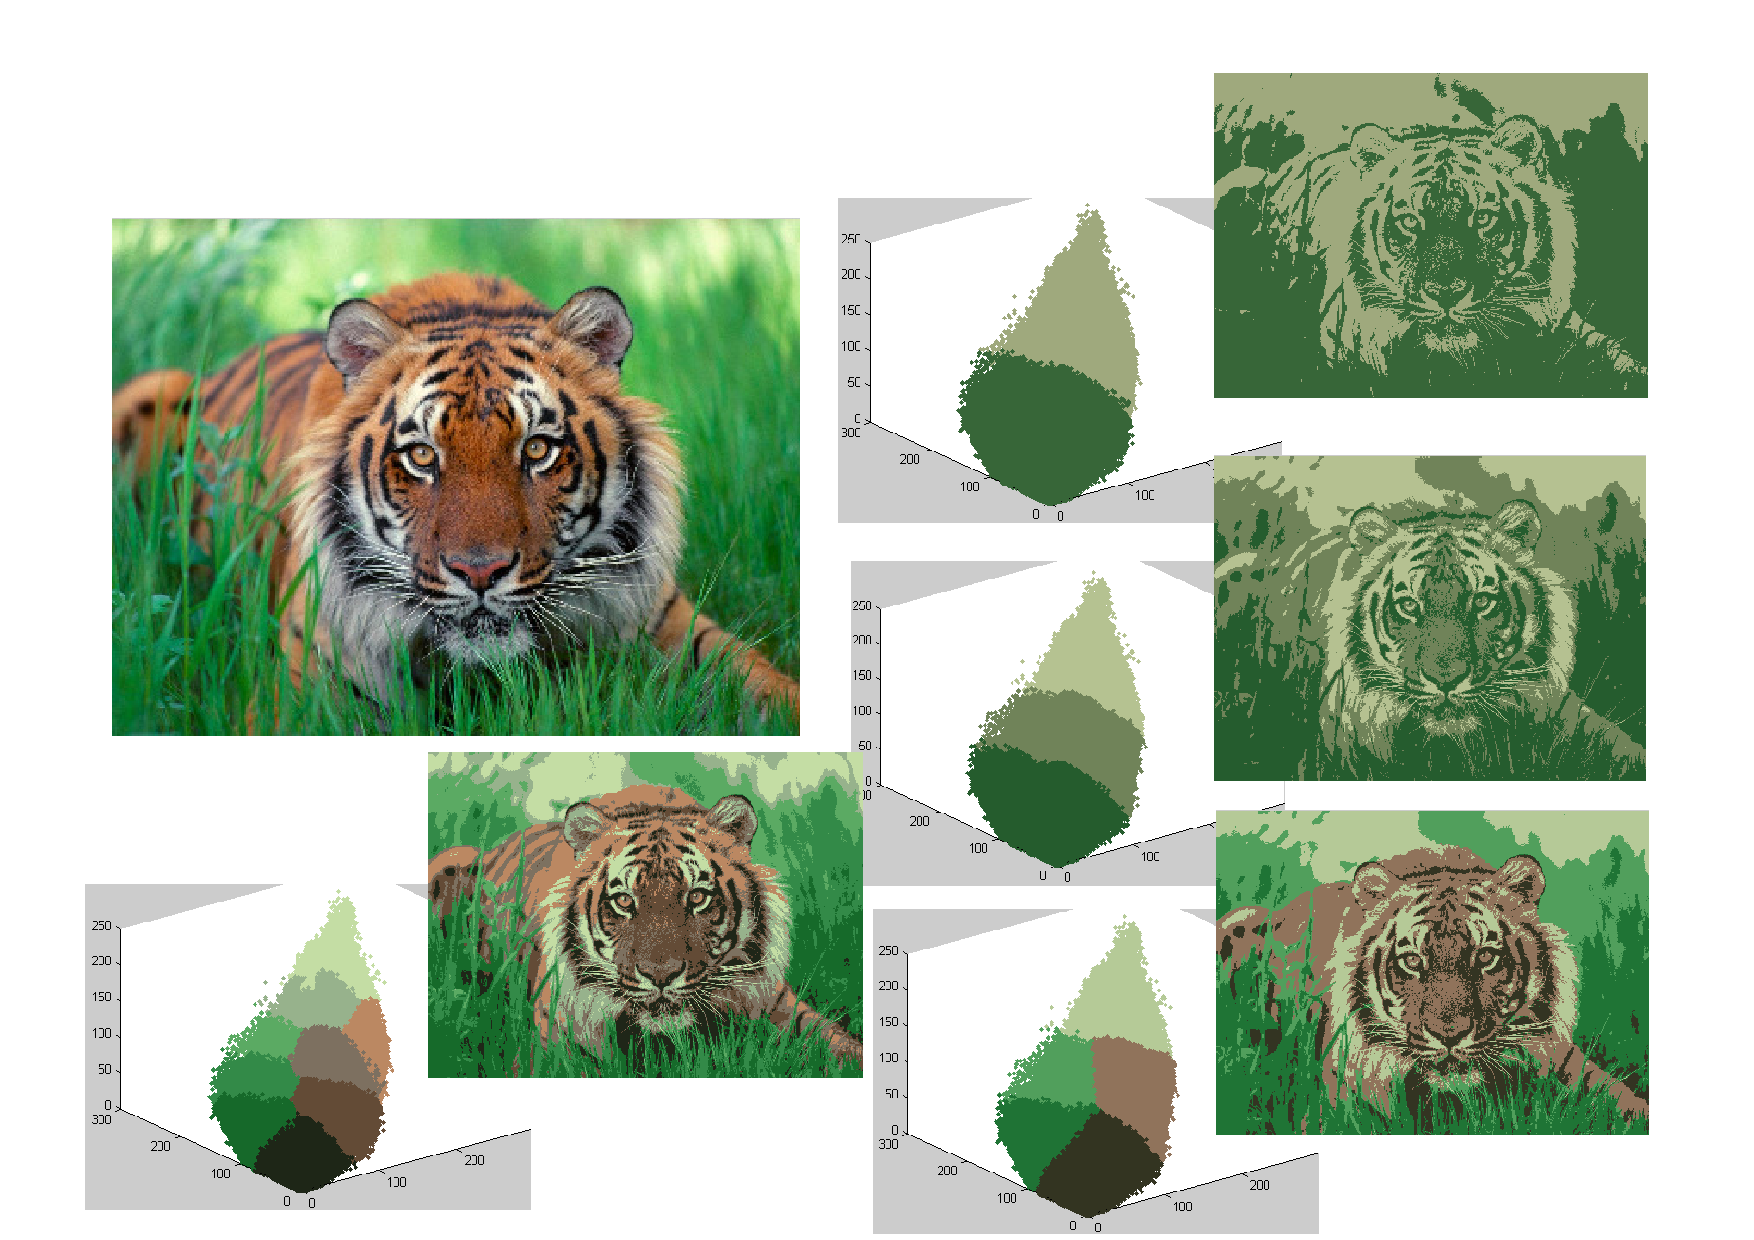
\includegraphics[angle=0,width=0.8\linewidth]{images/unsupervised/kmeans/kmeans_lion.pdf}
%				\caption{Single-Link Dendogram Good K}
			%\label{Enel_QQ_Plot_Normal}
		\end{figure}
%	\end{block}

\end{frame}


\begin{frame}

	\frametitle{{\color{GradientDescentDiagramBlue}Centroid-based Clustering}: segmentazione con il K-means}

%	\begin{block}{K-means: considerazioni}
		\begin{figure}[!htbp]
				\centering
				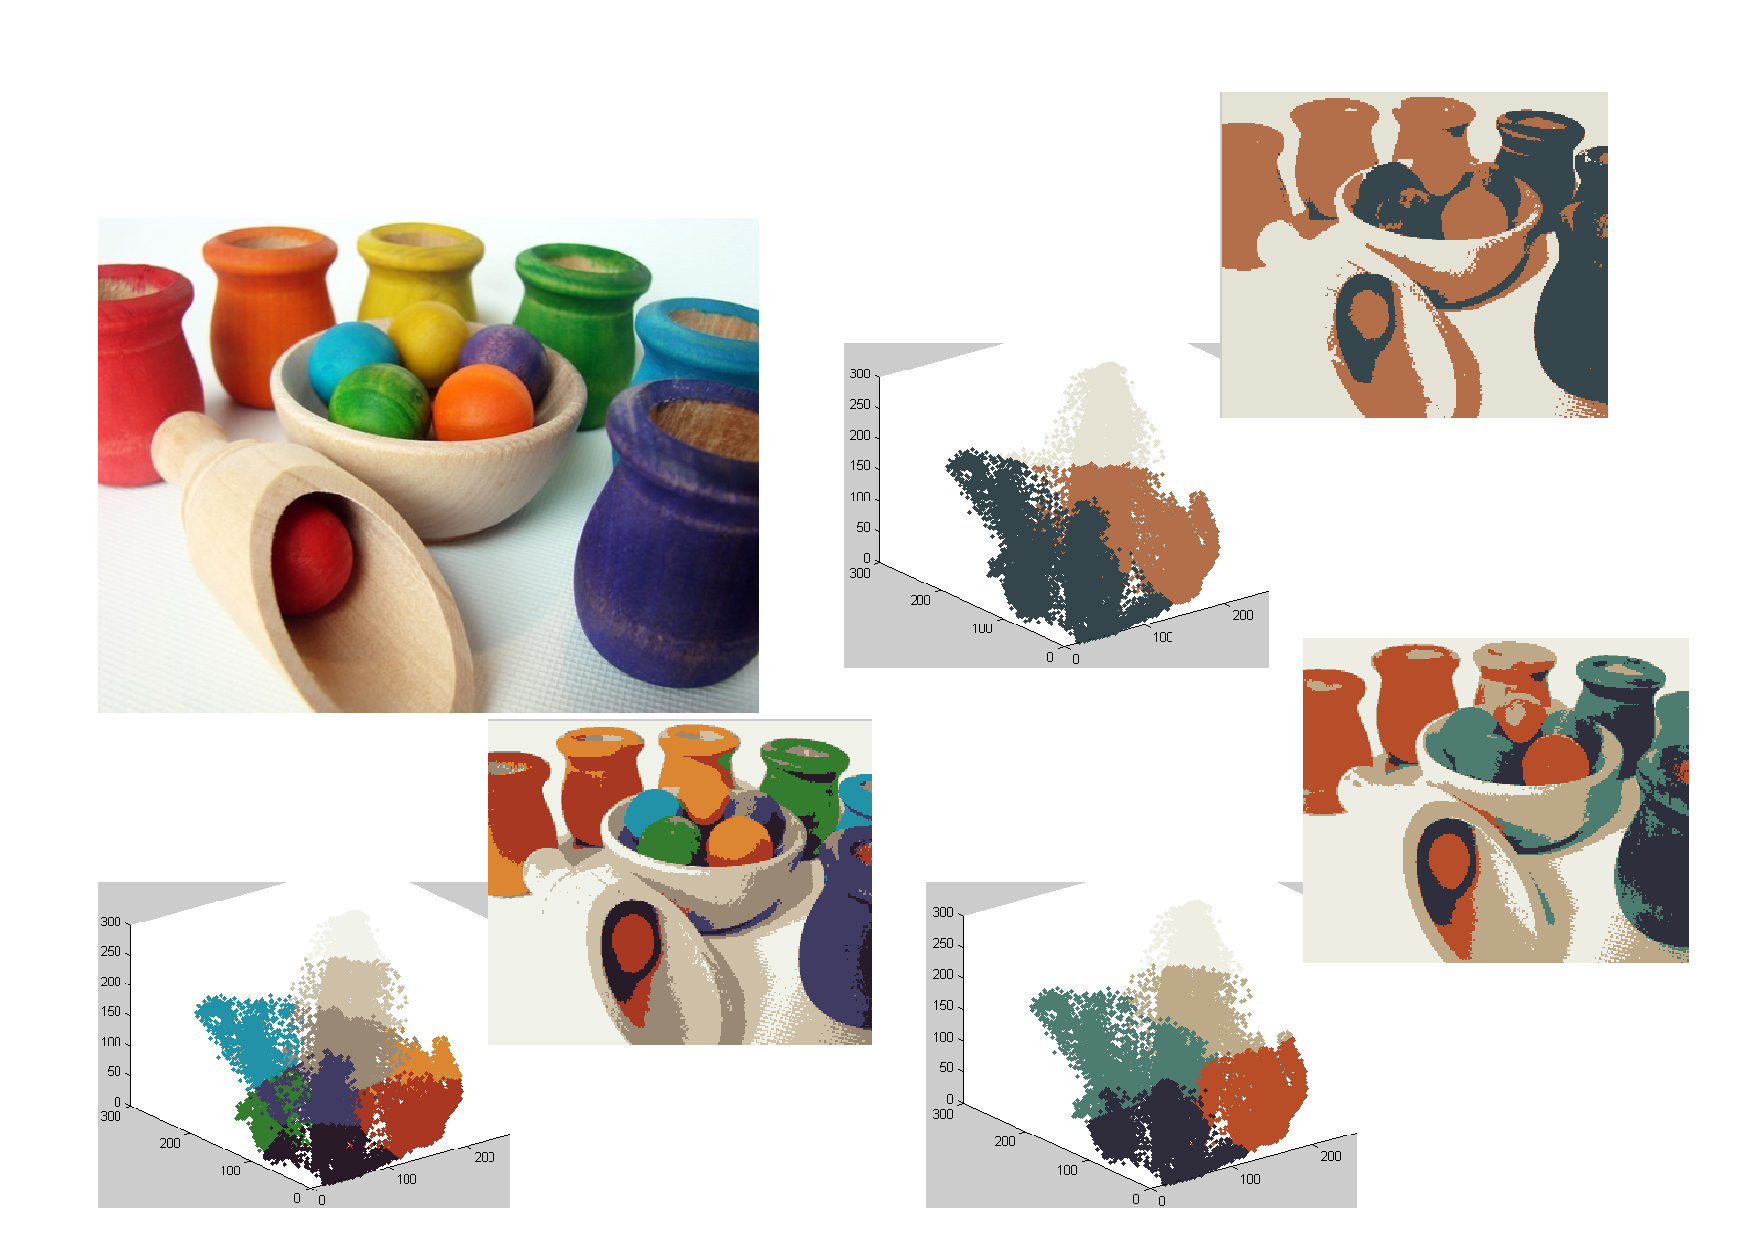
\includegraphics[angle=0,width=0.85\linewidth]{images/unsupervised/kmeans/kmeans_pots.pdf}
%				\caption{Single-Link Dendogram Good K}
				%\label{Enel_QQ_Plot_Normal}
			\end{figure}
%	\end{block}

\end{frame}
